% Festlegen des Dokumententyps
\documentclass[a4paper,twoside]{article}

% Papierformat
\usepackage{a4}

% Deutsche Sprache (Silbentrennung, usw.)
\usepackage[ngerman]{babel}

% Schrifteneinstellungen
\usepackage{lmodern}
\usepackage[T1]{fontenc}
\usepackage{textcomp}

% Kodierung
\usepackage{ucs}
\usepackage[utf8]{inputenc}

% bessere Matheunterstützung
\usepackage{amsfonts}
\usepackage{amstext}
\usepackage{amsmath}

% Einheiten in Formalen
\usepackage{siunitx}
\sisetup{%
locale=DE,
}

% fuer Zitate
\usepackage{cite}

% Grafiken einbinden
\usepackage{graphicx}


% Verweise in PDF-Dateien
\usepackage
[colorlinks,
pdfstartview = 1,
bookmarksopen = true,
bookmarksnumbered = true,
linkcolor = black,
plainpages = true,
hypertexnames = false,
citecolor = black]{hyperref} 

\newcommand{\e}{{\rm e}}

\begin{document}

\thispagestyle{empty}
\begin{center}
    {\Huge{\textbf{Physikalisches Praktikum}}}\\[16pt]
\ \\
\ \\
\ \\
\ \\
\ \\
\ \\
\ \\
\ \\
\ \\
\ \\
\ \\
\ \\
\ \\
\ \\
\ \\
\ \\
\ \\
\huge{Kreiselpräzession}
\ \\
\ \\
\large{Versuch 4}
\end{center}

\normalsize
\ \\
\ \\
\ \\
\ \\
\ \\

\begin{center}
\begin{tabular}{lcl}
      Name: & ~ & Timo Janßen \\
                    & ~ & E-Mail: timo.janssen1@stud.uni-goettingen.de \\
	  Mitarbeiter: & ~ & Tom Groß \\
		    & ~ & E-Mail: tom.gross@stud.uni-goettingen.de \\
\ \\		    
      Tutorin: & ~ & Jantje Freudenthal \\
      Gruppe: & ~ & 10 \\
\ \\      
      Durchgeführt am: & ~ & 27.05.2013 \\
      Protokoll abgegeben: & ~ & 10.06.2013 \\
      Protokoll verbessert: & ~ & ........................\\
\ \\
\ \\
      Testiert: .................................    
\end{tabular}\\
\end{center}

\newpage
%Seitennummerierung ausschalten
\thispagestyle{empty}
\tableofcontents
\newpage
%Seitenzähler zurücksetzen
\setcounter{page}{1}
\section{Auswertung}
\subsection{Schwingungen ohne Anregungen}
Nach der Aufbereitung der Messdaten kann zunächst der zeitliche Verlauf der nicht angeregten Schwingung für die verschiedenen Dämpfungen dargestellt werden (Abb. \ref{img:1}). Man erkennt deutlich das schnellere Abklingen bei stärkerer Dämpfung. 
Die Eigenfrequenz dieser Schwingungen bestimmt sich als Maximum der zugehörigen diskreten Fourier-Transformation (DFT) ~\cite[Rao, 2010]{FFT}. Die Ergebnisse sind in Tabelle \ref{tab:1} aufgetragen.
\begin{figure}[!htbp]
\centering
   % GNUPLOT: LaTeX picture with Postscript
\begingroup
  \makeatletter
  \providecommand\color[2][]{%
    \GenericError{(gnuplot) \space\space\space\@spaces}{%
      Package color not loaded in conjunction with
      terminal option `colourtext'%
    }{See the gnuplot documentation for explanation.%
    }{Either use 'blacktext' in gnuplot or load the package
      color.sty in LaTeX.}%
    \renewcommand\color[2][]{}%
  }%
  \providecommand\includegraphics[2][]{%
    \GenericError{(gnuplot) \space\space\space\@spaces}{%
      Package graphicx or graphics not loaded%
    }{See the gnuplot documentation for explanation.%
    }{The gnuplot epslatex terminal needs graphicx.sty or graphics.sty.}%
    \renewcommand\includegraphics[2][]{}%
  }%
  \providecommand\rotatebox[2]{#2}%
  \@ifundefined{ifGPcolor}{%
    \newif\ifGPcolor
    \GPcolortrue
  }{}%
  \@ifundefined{ifGPblacktext}{%
    \newif\ifGPblacktext
    \GPblacktexttrue
  }{}%
  % define a \g@addto@macro without @ in the name:
  \let\gplgaddtomacro\g@addto@macro
  % define empty templates for all commands taking text:
  \gdef\gplbacktext{}%
  \gdef\gplfronttext{}%
  \makeatother
  \ifGPblacktext
    % no textcolor at all
    \def\colorrgb#1{}%
    \def\colorgray#1{}%
  \else
    % gray or color?
    \ifGPcolor
      \def\colorrgb#1{\color[rgb]{#1}}%
      \def\colorgray#1{\color[gray]{#1}}%
      \expandafter\def\csname LTw\endcsname{\color{white}}%
      \expandafter\def\csname LTb\endcsname{\color{black}}%
      \expandafter\def\csname LTa\endcsname{\color{black}}%
      \expandafter\def\csname LT0\endcsname{\color[rgb]{1,0,0}}%
      \expandafter\def\csname LT1\endcsname{\color[rgb]{0,1,0}}%
      \expandafter\def\csname LT2\endcsname{\color[rgb]{0,0,1}}%
      \expandafter\def\csname LT3\endcsname{\color[rgb]{1,0,1}}%
      \expandafter\def\csname LT4\endcsname{\color[rgb]{0,1,1}}%
      \expandafter\def\csname LT5\endcsname{\color[rgb]{1,1,0}}%
      \expandafter\def\csname LT6\endcsname{\color[rgb]{0,0,0}}%
      \expandafter\def\csname LT7\endcsname{\color[rgb]{1,0.3,0}}%
      \expandafter\def\csname LT8\endcsname{\color[rgb]{0.5,0.5,0.5}}%
    \else
      % gray
      \def\colorrgb#1{\color{black}}%
      \def\colorgray#1{\color[gray]{#1}}%
      \expandafter\def\csname LTw\endcsname{\color{white}}%
      \expandafter\def\csname LTb\endcsname{\color{black}}%
      \expandafter\def\csname LTa\endcsname{\color{black}}%
      \expandafter\def\csname LT0\endcsname{\color{black}}%
      \expandafter\def\csname LT1\endcsname{\color{black}}%
      \expandafter\def\csname LT2\endcsname{\color{black}}%
      \expandafter\def\csname LT3\endcsname{\color{black}}%
      \expandafter\def\csname LT4\endcsname{\color{black}}%
      \expandafter\def\csname LT5\endcsname{\color{black}}%
      \expandafter\def\csname LT6\endcsname{\color{black}}%
      \expandafter\def\csname LT7\endcsname{\color{black}}%
      \expandafter\def\csname LT8\endcsname{\color{black}}%
    \fi
  \fi
  \setlength{\unitlength}{0.0500bp}%
  \begin{picture}(7200.00,5040.00)%
    \gplgaddtomacro\gplbacktext{%
      \csname LTb\endcsname%
      \put(948,3066){\makebox(0,0)[r]{\strut{}-1}}%
      \csname LTb\endcsname%
      \put(948,3360){\makebox(0,0)[r]{\strut{}-0.5}}%
      \csname LTb\endcsname%
      \put(948,3654){\makebox(0,0)[r]{\strut{}0}}%
      \csname LTb\endcsname%
      \put(948,3947){\makebox(0,0)[r]{\strut{}0.5}}%
      \csname LTb\endcsname%
      \put(948,4241){\makebox(0,0)[r]{\strut{}1}}%
      \csname LTb\endcsname%
      \put(1080,2552){\makebox(0,0){\strut{}}}%
      \csname LTb\endcsname%
      \put(1656,2552){\makebox(0,0){\strut{}}}%
      \csname LTb\endcsname%
      \put(2232,2552){\makebox(0,0){\strut{}}}%
      \csname LTb\endcsname%
      \put(2807,2552){\makebox(0,0){\strut{}}}%
      \csname LTb\endcsname%
      \put(3383,2552){\makebox(0,0){\strut{}}}%
      \put(178,3653){\rotatebox{-270}{\makebox(0,0){\strut{}$\varphi/\varphi_0$}}}%
    }%
    \gplgaddtomacro\gplfronttext{%
      \csname LTb\endcsname%
      \put(2972,4362){\makebox(0,0)[r]{\strut{}Dämpfung 0mm}}%
    }%
    \gplgaddtomacro\gplbacktext{%
      \csname LTb\endcsname%
      \put(3828,3066){\makebox(0,0)[r]{\strut{}}}%
      \csname LTb\endcsname%
      \put(3828,3360){\makebox(0,0)[r]{\strut{}}}%
      \csname LTb\endcsname%
      \put(3828,3654){\makebox(0,0)[r]{\strut{}}}%
      \csname LTb\endcsname%
      \put(3828,3947){\makebox(0,0)[r]{\strut{}}}%
      \csname LTb\endcsname%
      \put(3828,4241){\makebox(0,0)[r]{\strut{}}}%
      \csname LTb\endcsname%
      \put(3960,2552){\makebox(0,0){\strut{}}}%
      \csname LTb\endcsname%
      \put(4536,2552){\makebox(0,0){\strut{}}}%
      \csname LTb\endcsname%
      \put(5112,2552){\makebox(0,0){\strut{}}}%
      \csname LTb\endcsname%
      \put(5687,2552){\makebox(0,0){\strut{}}}%
      \csname LTb\endcsname%
      \put(6263,2552){\makebox(0,0){\strut{}}}%
    }%
    \gplgaddtomacro\gplfronttext{%
      \csname LTb\endcsname%
      \put(5852,4362){\makebox(0,0)[r]{\strut{}Dämpfung 4mm}}%
    }%
    \gplgaddtomacro\gplbacktext{%
      \csname LTb\endcsname%
      \put(948,1302){\makebox(0,0)[r]{\strut{}-1}}%
      \csname LTb\endcsname%
      \put(948,1596){\makebox(0,0)[r]{\strut{}-0.5}}%
      \csname LTb\endcsname%
      \put(948,1890){\makebox(0,0)[r]{\strut{}0}}%
      \csname LTb\endcsname%
      \put(948,2183){\makebox(0,0)[r]{\strut{}0.5}}%
      \csname LTb\endcsname%
      \put(948,2477){\makebox(0,0)[r]{\strut{}1}}%
      \csname LTb\endcsname%
      \put(1080,788){\makebox(0,0){\strut{}0}}%
      \csname LTb\endcsname%
      \put(1656,788){\makebox(0,0){\strut{}5}}%
      \csname LTb\endcsname%
      \put(2232,788){\makebox(0,0){\strut{}10}}%
      \csname LTb\endcsname%
      \put(2807,788){\makebox(0,0){\strut{}15}}%
      \csname LTb\endcsname%
      \put(3383,788){\makebox(0,0){\strut{}20}}%
      \put(178,1889){\rotatebox{-270}{\makebox(0,0){\strut{}$\varphi/\varphi_0$}}}%
      \put(2519,458){\makebox(0,0){\strut{}$t [s]$}}%
    }%
    \gplgaddtomacro\gplfronttext{%
      \csname LTb\endcsname%
      \put(2972,2598){\makebox(0,0)[r]{\strut{}Dämpfung 6mm}}%
    }%
    \gplgaddtomacro\gplbacktext{%
      \csname LTb\endcsname%
      \put(3828,1302){\makebox(0,0)[r]{\strut{}}}%
      \csname LTb\endcsname%
      \put(3828,1596){\makebox(0,0)[r]{\strut{}}}%
      \csname LTb\endcsname%
      \put(3828,1890){\makebox(0,0)[r]{\strut{}}}%
      \csname LTb\endcsname%
      \put(3828,2183){\makebox(0,0)[r]{\strut{}}}%
      \csname LTb\endcsname%
      \put(3828,2477){\makebox(0,0)[r]{\strut{}}}%
      \csname LTb\endcsname%
      \put(3960,788){\makebox(0,0){\strut{}0}}%
      \csname LTb\endcsname%
      \put(4536,788){\makebox(0,0){\strut{}5}}%
      \csname LTb\endcsname%
      \put(5112,788){\makebox(0,0){\strut{}10}}%
      \csname LTb\endcsname%
      \put(5687,788){\makebox(0,0){\strut{}15}}%
      \csname LTb\endcsname%
      \put(6263,788){\makebox(0,0){\strut{}20}}%
      \put(5399,458){\makebox(0,0){\strut{}$t [s]$}}%
    }%
    \gplgaddtomacro\gplfronttext{%
      \csname LTb\endcsname%
      \put(5852,2598){\makebox(0,0)[r]{\strut{}Dämpfung 8mm}}%
    }%
    \gplbacktext
    \put(0,0){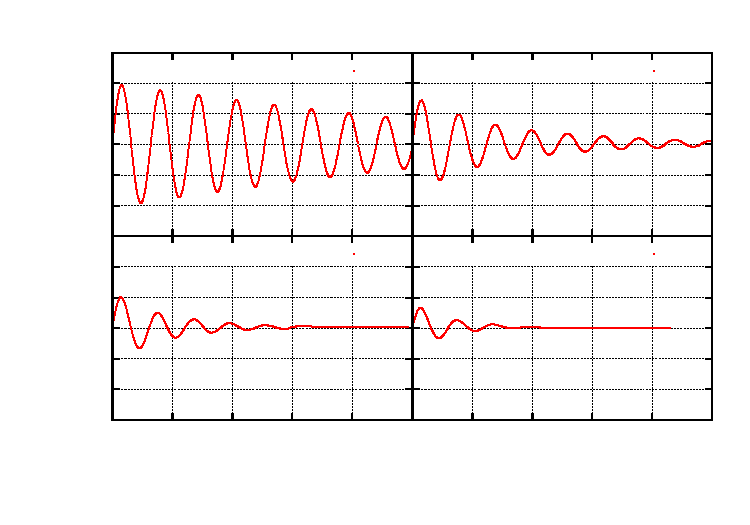
\includegraphics{plot_dif0}}%
    \gplfronttext
  \end{picture}%
\endgroup

   \caption{\small{Schwingungsverlauf des Pohlschen Rades ohne Anregung für vier verschiedene Dämpfungen}}
   \label{img:1}
\end{figure}
\ \\
Mit der Gleichung
\begin{align}
\Lambda := \rm {ln}\left[{\frac{\varphi(t)}{\varphi(t+T)}}\right]=\beta T \nonumber
\end{align}
kann das Logarithmische Dekrement berechnet werden. Dazu werden mit einem Peakfinding-Algorithmus die Maxima der Schwingung bestimmt und jeweils für zwei benachbarte Maxima das Logarithmische Dekrement berechnet. Anschließend werden die Werte gemittelt. Die Dämpfung $\beta$ ergibt sich dann durch Multiplikation mit der Periodendauer. Die Ergebnisse befinden sich ebenfalls in Tabelle \ref{tab:1}.\\
Damit lässt sich nun die ungedämpfte Eigenfrequenz über die Beziehung
\begin{align}
\omega_e = \sqrt{\omega_0^{2}-\beta^{2}}  \Leftrightarrow \omega_0 = \sqrt{\omega_e^{2}+\beta^{2}}
\end{align}
finden. Der Mittelwert über die vier Messungen ist
\begin{align}
\omega_0 = \SI{2,08\pm0,18}{\per\second} \nonumber
\end{align}
Dieser stimmt nicht überein mit der Eigenfrequenz für die Stellung "`0 mm"' der Wirbelstrombremse. Dies ist aber nicht verwunderlich, wenn man bedenkt, dass das betrachtete System selbst bei abgeschalteter Wirbelstrombremse nicht völlig reibungs- bzw. dämpfungsfrei ist. Es treten sowohl Luftreibung, als auch mechanische Reibung in den Lagern auf, was sich auch im Wert der Dämpfungskonstante niederschlägt.
\begin{table}[!htbp]
\centering
\begin{tabular}{|l|l|l|l|l|}
\hline 
Dämpfung & $\SI{0}{mm}$ & $\SI{4}{mm}$ & $\SI{6}{mm}$ & $\SI{8}{mm}$ \\
\hline
$\omega_e$ $[\SI{}{\per\second}]$ & $\SI{2,06\pm0,10}{\per\second}$ & $\SI{2,06\pm0,10}{\per\second}$ & $\SI{2,16\pm0,13}{\per\second}$ & $\SI{1,96\pm0,15}{\per\second}$ \\
\hline
$\Lambda$ & $\SI{0,112\pm0,005}{}$ & $\SI{0,38\pm0,06}{}$ & $\SI{0,80\pm0,06}{}$ & $\SI{1,5\pm0,4}{}$ \\
\hline
$\beta$ $[\SI{}{\per\second}]$ & \SI{0,037\pm0,005}{} & \SI{0,12\pm0,06}{} & \SI{0,27\pm0,06}{} & \SI{0,5\pm0,4}{} \\
%\hline
%Errechnete & & & & \\ ungedämpfte & & & & \\  Eigenfrequenz & & & & \\$\omega_0$: & ... & ... & ... & \\
\hline 
\end{tabular} 
\caption{\small{Auswertung der Schwingungen für die vier Dämpfungen ohne Anregung}}
\label{tab:1}
\end{table}
\newpage
\subsection{Schwingungen mit Anregungen}
Zunächst soll für jede Dämpfung die Resonanzkurve aufgetragen werden. Dazu  muss für jede Kombination aus Dämpfung und Erregerfrequenz die Schwingungsamplitude bestimmt werden. Dies geschieht durch Suchen der Minima/Maxima mit dem bereits erwähnten Peakfinding-Algorithmus und anschließende Mittelwertbildung. Abbildung \ref{img:2} zeigt die resultierenden Kurven für alle Dämpfungen:
\ \\
\begin{figure}[!htbp]
\centering
% GNUPLOT: LaTeX picture with Postscript
\begingroup
  \makeatletter
  \providecommand\color[2][]{%
    \GenericError{(gnuplot) \space\space\space\@spaces}{%
      Package color not loaded in conjunction with
      terminal option `colourtext'%
    }{See the gnuplot documentation for explanation.%
    }{Either use 'blacktext' in gnuplot or load the package
      color.sty in LaTeX.}%
    \renewcommand\color[2][]{}%
  }%
  \providecommand\includegraphics[2][]{%
    \GenericError{(gnuplot) \space\space\space\@spaces}{%
      Package graphicx or graphics not loaded%
    }{See the gnuplot documentation for explanation.%
    }{The gnuplot epslatex terminal needs graphicx.sty or graphics.sty.}%
    \renewcommand\includegraphics[2][]{}%
  }%
  \providecommand\rotatebox[2]{#2}%
  \@ifundefined{ifGPcolor}{%
    \newif\ifGPcolor
    \GPcolortrue
  }{}%
  \@ifundefined{ifGPblacktext}{%
    \newif\ifGPblacktext
    \GPblacktexttrue
  }{}%
  % define a \g@addto@macro without @ in the name:
  \let\gplgaddtomacro\g@addto@macro
  % define empty templates for all commands taking text:
  \gdef\gplbacktext{}%
  \gdef\gplfronttext{}%
  \makeatother
  \ifGPblacktext
    % no textcolor at all
    \def\colorrgb#1{}%
    \def\colorgray#1{}%
  \else
    % gray or color?
    \ifGPcolor
      \def\colorrgb#1{\color[rgb]{#1}}%
      \def\colorgray#1{\color[gray]{#1}}%
      \expandafter\def\csname LTw\endcsname{\color{white}}%
      \expandafter\def\csname LTb\endcsname{\color{black}}%
      \expandafter\def\csname LTa\endcsname{\color{black}}%
      \expandafter\def\csname LT0\endcsname{\color[rgb]{1,0,0}}%
      \expandafter\def\csname LT1\endcsname{\color[rgb]{0,1,0}}%
      \expandafter\def\csname LT2\endcsname{\color[rgb]{0,0,1}}%
      \expandafter\def\csname LT3\endcsname{\color[rgb]{1,0,1}}%
      \expandafter\def\csname LT4\endcsname{\color[rgb]{0,1,1}}%
      \expandafter\def\csname LT5\endcsname{\color[rgb]{1,1,0}}%
      \expandafter\def\csname LT6\endcsname{\color[rgb]{0,0,0}}%
      \expandafter\def\csname LT7\endcsname{\color[rgb]{1,0.3,0}}%
      \expandafter\def\csname LT8\endcsname{\color[rgb]{0.5,0.5,0.5}}%
    \else
      % gray
      \def\colorrgb#1{\color{black}}%
      \def\colorgray#1{\color[gray]{#1}}%
      \expandafter\def\csname LTw\endcsname{\color{white}}%
      \expandafter\def\csname LTb\endcsname{\color{black}}%
      \expandafter\def\csname LTa\endcsname{\color{black}}%
      \expandafter\def\csname LT0\endcsname{\color{black}}%
      \expandafter\def\csname LT1\endcsname{\color{black}}%
      \expandafter\def\csname LT2\endcsname{\color{black}}%
      \expandafter\def\csname LT3\endcsname{\color{black}}%
      \expandafter\def\csname LT4\endcsname{\color{black}}%
      \expandafter\def\csname LT5\endcsname{\color{black}}%
      \expandafter\def\csname LT6\endcsname{\color{black}}%
      \expandafter\def\csname LT7\endcsname{\color{black}}%
      \expandafter\def\csname LT8\endcsname{\color{black}}%
    \fi
  \fi
  \setlength{\unitlength}{0.0500bp}%
  \begin{picture}(7200.00,5040.00)%
    \gplgaddtomacro\gplbacktext{%
      \csname LTb\endcsname%
      \put(682,704){\makebox(0,0)[r]{\strut{} 0}}%
      \put(682,1213){\makebox(0,0)[r]{\strut{} 1}}%
      \put(682,1722){\makebox(0,0)[r]{\strut{} 2}}%
      \put(682,2231){\makebox(0,0)[r]{\strut{} 3}}%
      \put(682,2740){\makebox(0,0)[r]{\strut{} 4}}%
      \put(682,3248){\makebox(0,0)[r]{\strut{} 5}}%
      \put(682,3757){\makebox(0,0)[r]{\strut{} 6}}%
      \put(682,4266){\makebox(0,0)[r]{\strut{} 7}}%
      \put(682,4775){\makebox(0,0)[r]{\strut{} 8}}%
      \put(814,484){\makebox(0,0){\strut{} 0}}%
      \put(2311,484){\makebox(0,0){\strut{} 0.5}}%
      \put(3809,484){\makebox(0,0){\strut{} 1}}%
      \put(5306,484){\makebox(0,0){\strut{} 1.5}}%
      \put(6803,484){\makebox(0,0){\strut{} 2}}%
      \put(176,2739){\rotatebox{-270}{\makebox(0,0){\strut{}$\phi_0(\omega)/\phi_0(0)$}}}%
      \put(3808,154){\makebox(0,0){\strut{}$\omega/\omega_0$}}%
    }%
    \gplgaddtomacro\gplfronttext{%
      \csname LTb\endcsname%
      \put(5816,4602){\makebox(0,0)[r]{\strut{}4mm}}%
      \csname LTb\endcsname%
      \put(5816,4382){\makebox(0,0)[r]{\strut{}6mm}}%
      \csname LTb\endcsname%
      \put(5816,4162){\makebox(0,0)[r]{\strut{}8mm}}%
    }%
    \gplbacktext
    \put(0,0){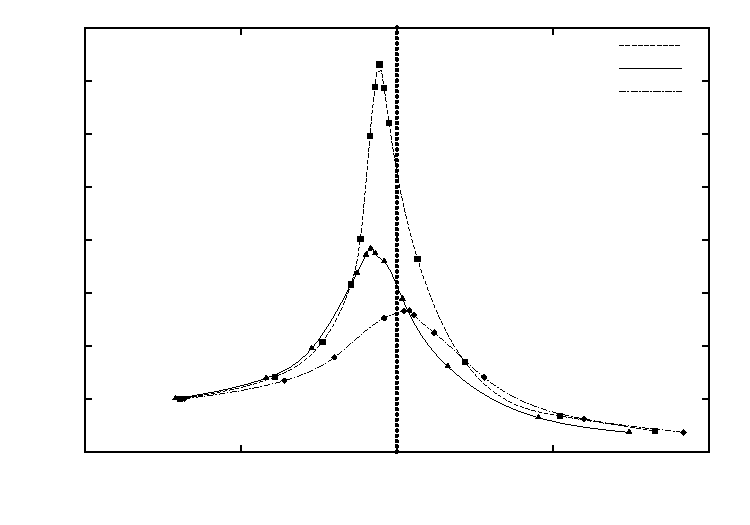
\includegraphics{frequenzgang}}%
    \gplfronttext
  \end{picture}%
\endgroup

\caption{Das unterschiedliche Resonanzverhalten des Rades für die drei Dämpfungen in Abhängigkeit von Eigenfrequenz
und Anregungsfrequenz} 
\label{img:2}
\end{figure}
\newpage \ \\
Durch die externe Anregung des Resonators entsteht eine Phasenverschiebung $\phi$, die von der Dämpfung und der Erregerfrequenz abhängt:
\begin{align}
\phi=arctan\left(\frac{2\beta\omega}{\omega_0^{2}-\omega^{2}}\right) \nonumber
\end{align}
Trägt man die Phasenverschiebung (im Bereich zwischen 0° und 180°) gegen das Verhältnis von der Erregerfrequenz zur Eigenfrequenz des Systems auf, erhält man folgende Darstellung:
\begin{figure}[!htbp]
% GNUPLOT: LaTeX picture with Postscript
\begingroup
  \makeatletter
  \providecommand\color[2][]{%
    \GenericError{(gnuplot) \space\space\space\@spaces}{%
      Package color not loaded in conjunction with
      terminal option `colourtext'%
    }{See the gnuplot documentation for explanation.%
    }{Either use 'blacktext' in gnuplot or load the package
      color.sty in LaTeX.}%
    \renewcommand\color[2][]{}%
  }%
  \providecommand\includegraphics[2][]{%
    \GenericError{(gnuplot) \space\space\space\@spaces}{%
      Package graphicx or graphics not loaded%
    }{See the gnuplot documentation for explanation.%
    }{The gnuplot epslatex terminal needs graphicx.sty or graphics.sty.}%
    \renewcommand\includegraphics[2][]{}%
  }%
  \providecommand\rotatebox[2]{#2}%
  \@ifundefined{ifGPcolor}{%
    \newif\ifGPcolor
    \GPcolortrue
  }{}%
  \@ifundefined{ifGPblacktext}{%
    \newif\ifGPblacktext
    \GPblacktexttrue
  }{}%
  % define a \g@addto@macro without @ in the name:
  \let\gplgaddtomacro\g@addto@macro
  % define empty templates for all commands taking text:
  \gdef\gplbacktext{}%
  \gdef\gplfronttext{}%
  \makeatother
  \ifGPblacktext
    % no textcolor at all
    \def\colorrgb#1{}%
    \def\colorgray#1{}%
  \else
    % gray or color?
    \ifGPcolor
      \def\colorrgb#1{\color[rgb]{#1}}%
      \def\colorgray#1{\color[gray]{#1}}%
      \expandafter\def\csname LTw\endcsname{\color{white}}%
      \expandafter\def\csname LTb\endcsname{\color{black}}%
      \expandafter\def\csname LTa\endcsname{\color{black}}%
      \expandafter\def\csname LT0\endcsname{\color[rgb]{1,0,0}}%
      \expandafter\def\csname LT1\endcsname{\color[rgb]{0,1,0}}%
      \expandafter\def\csname LT2\endcsname{\color[rgb]{0,0,1}}%
      \expandafter\def\csname LT3\endcsname{\color[rgb]{1,0,1}}%
      \expandafter\def\csname LT4\endcsname{\color[rgb]{0,1,1}}%
      \expandafter\def\csname LT5\endcsname{\color[rgb]{1,1,0}}%
      \expandafter\def\csname LT6\endcsname{\color[rgb]{0,0,0}}%
      \expandafter\def\csname LT7\endcsname{\color[rgb]{1,0.3,0}}%
      \expandafter\def\csname LT8\endcsname{\color[rgb]{0.5,0.5,0.5}}%
    \else
      % gray
      \def\colorrgb#1{\color{black}}%
      \def\colorgray#1{\color[gray]{#1}}%
      \expandafter\def\csname LTw\endcsname{\color{white}}%
      \expandafter\def\csname LTb\endcsname{\color{black}}%
      \expandafter\def\csname LTa\endcsname{\color{black}}%
      \expandafter\def\csname LT0\endcsname{\color{black}}%
      \expandafter\def\csname LT1\endcsname{\color{black}}%
      \expandafter\def\csname LT2\endcsname{\color{black}}%
      \expandafter\def\csname LT3\endcsname{\color{black}}%
      \expandafter\def\csname LT4\endcsname{\color{black}}%
      \expandafter\def\csname LT5\endcsname{\color{black}}%
      \expandafter\def\csname LT6\endcsname{\color{black}}%
      \expandafter\def\csname LT7\endcsname{\color{black}}%
      \expandafter\def\csname LT8\endcsname{\color{black}}%
    \fi
  \fi
  \setlength{\unitlength}{0.0500bp}%
  \begin{picture}(7200.00,5040.00)%
    \gplgaddtomacro\gplbacktext{%
      \csname LTb\endcsname%
      \put(946,704){\makebox(0,0)[r]{\strut{} 0}}%
      \csname LTb\endcsname%
      \put(946,1518){\makebox(0,0)[r]{\strut{} 0.2}}%
      \csname LTb\endcsname%
      \put(946,2332){\makebox(0,0)[r]{\strut{} 0.4}}%
      \csname LTb\endcsname%
      \put(946,3147){\makebox(0,0)[r]{\strut{} 0.6}}%
      \csname LTb\endcsname%
      \put(946,3961){\makebox(0,0)[r]{\strut{} 0.8}}%
      \csname LTb\endcsname%
      \put(946,4775){\makebox(0,0)[r]{\strut{} 1}}%
      \csname LTb\endcsname%
      \put(1078,484){\makebox(0,0){\strut{} 0}}%
      \csname LTb\endcsname%
      \put(2509,484){\makebox(0,0){\strut{} 0.5}}%
      \csname LTb\endcsname%
      \put(3941,484){\makebox(0,0){\strut{} 1}}%
      \csname LTb\endcsname%
      \put(5372,484){\makebox(0,0){\strut{} 1.5}}%
      \csname LTb\endcsname%
      \put(6803,484){\makebox(0,0){\strut{} 2}}%
      \put(176,2739){\rotatebox{-270}{\makebox(0,0){\strut{}$\phi/\pi$}}}%
      \put(3940,154){\makebox(0,0){\strut{}$\omega/\omega_0$}}%
    }%
    \gplgaddtomacro\gplfronttext{%
      \csname LTb\endcsname%
      \put(5816,1317){\makebox(0,0)[r]{\strut{}4mm}}%
      \csname LTb\endcsname%
      \put(5816,1097){\makebox(0,0)[r]{\strut{}6mm}}%
      \csname LTb\endcsname%
      \put(5816,877){\makebox(0,0)[r]{\strut{}8mm}}%
    }%
    \gplbacktext
    \put(0,0){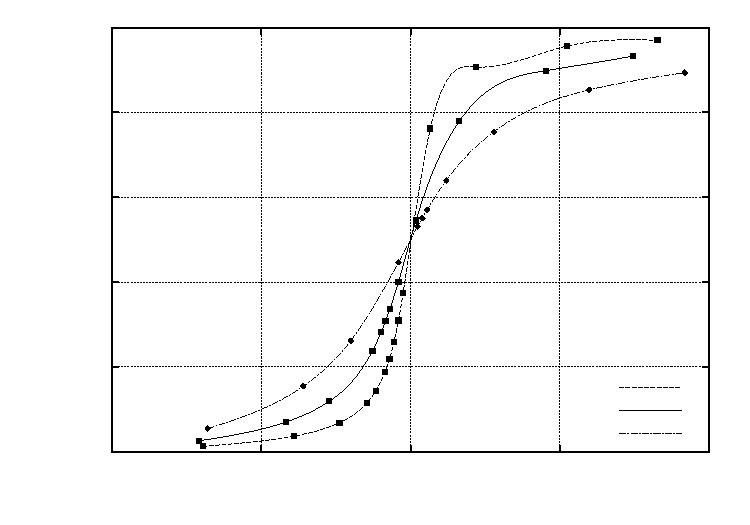
\includegraphics{phasenverschiebung}}%
    \gplfronttext
  \end{picture}%
\endgroup

\caption{Die unterschiedlichen Phasenverschiebungen des Rades abhängig vom Verhältnis von Eigenfrequenz zu 
Anregungsfrequenz}{Anmerkung: Durch die Annäherung mit Splines entspricht der Kurvenverlauf teilweise nicht der Theorie} 
\end{figure}
\newpage \ \\
Aus Abb. \ref{img:2} lassen sich die gemessenen Resonanzfrequenzen bestimmen. Die theoretisch erwarteten Resonanzfrequenzen lassen sich aus den gemessenen Dämpfungskonstanten und Eigenfrequenzen über die Formel
\begin{align}
\omega_r = \sqrt{\omega_0^{2} - 2\beta^{2}} \nonumber
\end{align}
berechnen. Der Vergleich in Tab. \ref{tab:2} zeigt, dass die Werte im Rahmen der Fehlergenauigkeit übereinstimmen. Dies liegt zum Teil auch an den relativ großen Fehlern der berechneten Werte, welche aus der Bestimmung des Logarithmischen Dekrements resultieren. Auffällig ist, dass die erwarteten Werte mit zunehmender Dämpfung tendenziell abfallen, während die gemessenen Werte tendenziell größer werden. 
\begin{table}[!htbp]
\centering
\begin{tabular}{|c|c|c|}
\hline 
Stellung der Wirbelstrombremse & $\omega_r$ erwartet & $\omega_r$ gemessen \\ 
\hline 
$\SI{4}{mm}$ & $\SI{2.1\pm0.4}{\per\second}$ & $\SI{1.95\pm0.10}{\per\second}$ \\ 
\hline 
$\SI{6}{mm}$ & $\SI{2.1\pm0.4}{\per\second}$ & $\SI{1.98\pm0.13}{\per\second}$ \\ 
\hline 
$\SI{8}{mm}$ & $\SI{1.8\pm0.7}{\per\second}$ & $\SI{2.04\pm0.15}{\per\second}$ \\ 
\hline 
\end{tabular} 
\caption{\small{Vergleich der erwarteten und der gemessenen Resonanzfrequenzen}}
\label{tab:2}
\end{table}
\newpage
\newpage
\thispagestyle{empty}
% Festlegung Art der Zitierung - Havardmethode: Abkuerzung Autor + Jahr
\bibliographystyle{plain}
\end{document}